\section{Introduction}
In 2000, Wood publishes a paper: The Feasibility of Magnetic Recording at 1 Terabits Per Square Inch~\cite{Wood2000}. It says, that conventional recording would reach a limit at around 1 Terabit/in$^2$.

However, in 2009, he admits~\cite{Wood2009} the current hard disk drive (HDD) technology is already reaching this limit. Wood is right that to assure continued capacity growth in HDD need alternative technologies: heat-assisted magnetic recording (HAMR)~\cite{Rottmeyer} and bit patterned media (BPM)~\cite{Terris}. 

Toward proof of the concept, the Advanced Storage Technology Consortium (ASTC)~\cite{ASTC} released the 2014 roadmap for HDD area density as shown in Fig.\,\ref{fig_astc}.

As you can see from Fig.~\,\ref{fig_astc}, current HDD technology is Perpendicular recording\

\begin{figure}[!hbt]
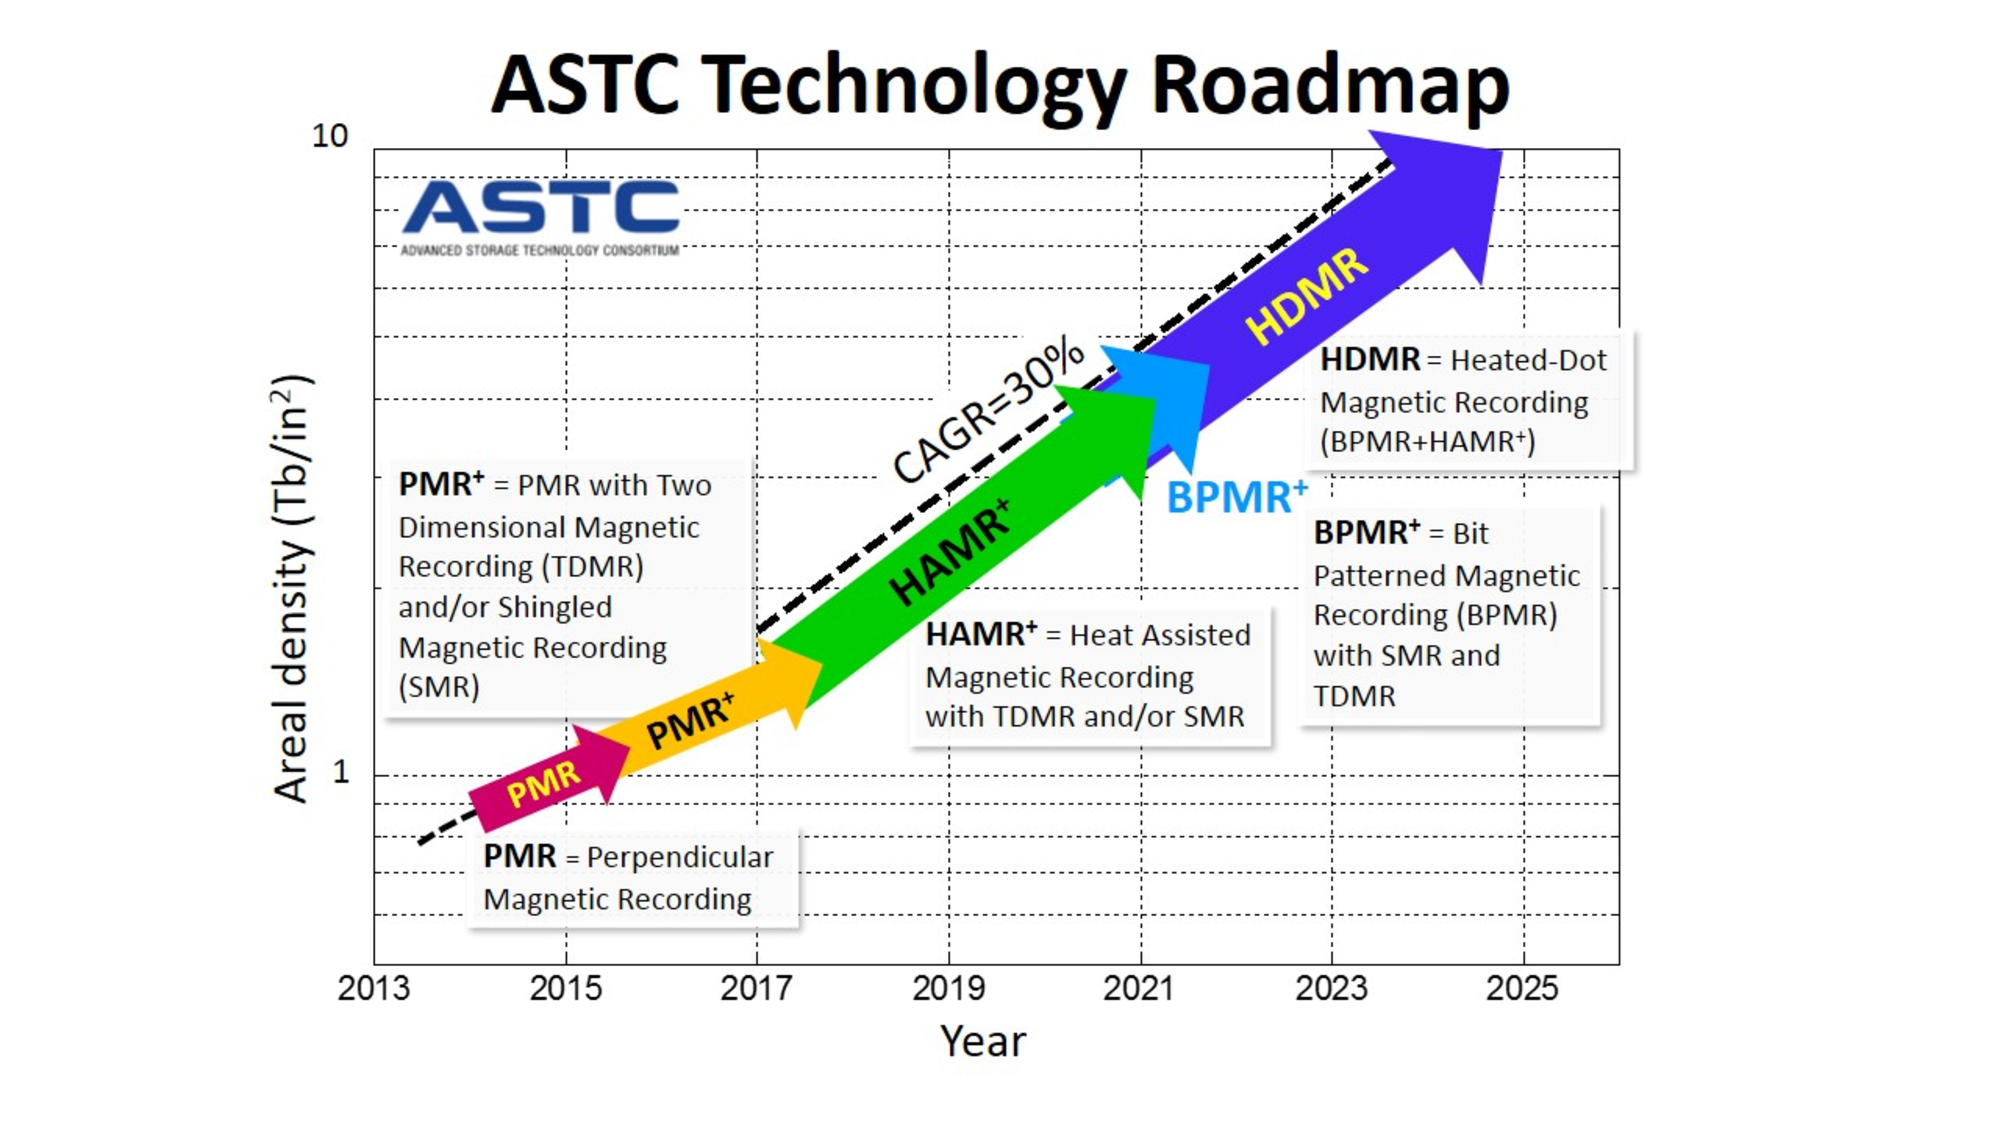
\includegraphics[height=0.25\textheight]{ASTC}
\caption{Data synchronization between two devices}
\label{fig_astc}
\end{figure}